\documentclass[hidelinks,a4paper,12pt]{article}
\usepackage[english]{babel}
\usepackage[utf8]{inputenc}
\usepackage{csquotes}
\usepackage{graphicx}
\usepackage{makecell}
\usepackage[margin=0.7in]{geometry}
\usepackage[T1]{fontenc}
\usepackage{mathptmx}
\usepackage{hyperref}
\hypersetup{
    colorlinks=false,
    linkcolor=blue,
    filecolor=magenta,      
    urlcolor=cyan,
}
\usepackage[normalem]{ulem}
\usepackage{xcolor}

\renewcommand\theadalign{bc}
\renewcommand\theadfont{\bfseries}
\renewcommand\theadgape{\Gape[4pt]}
\renewcommand\cellgape{\Gape[4pt]}
\graphicspath{ {./images/} }

\usepackage{comment}
  
\usepackage[backend=biber,style=numeric-comp,sorting=none,]{biblatex}
\addbibresource{references.bib} %Imports bibliography file

%opening
\title{Software Proposal Document for Candy Cake Page}
\author{Team Leader name, Tsneam Ahmed Eliwa Zky , Third Name, Fourth Name, Fifth Name \\
Supervised by: Dr. Essam Eliwa, Eng. Omar Magdy}


\begin{document}
\maketitle
\begin{table}[ht]

\caption{Document version history}
\begin{tabular}{|l|l|l|}
\hline
\thead{Proposal Version}    & \thead{Date} & \thead{Reason for Change}  \\ \hline
1.0 & 25-Feb-2023   & \makecell{Proposal First version’s specifications are defined}   \\ \hline
1.1 & 28-Feb-2023   & \makecell{System description updated} \\ \hline
\end{tabular}

\end{table}

\begin{table}[ht]
\begin{tabular}{cc}
\thead{GitHub:}    & {........................................................}   
\end{tabular}
\end{table}

\medskip

\begin{abstract}
The abstract should be concise and compelling, providing a compelling summary that encourages the reader to continue reading the full proposal document. It should briefly overview the proposed software project, including its purpose, scope, and critical features. It should give the reader a clear understanding of the project's objectives and benefits and any unique aspects that set it apart from similar software solutions.
The abstract should also include information about the software's target audience or user group and any relevant market or industry trends that make the project particularly timely.
In addition, the abstract may summarize key technical details such as the software's architecture, programming language, development methodology, and testing procedures. It may also mention any significant risks or challenges associated with the project and the strategies proposed to mitigate them.

To write a good abstract you can follow this guideline:

\begin{itemize}
    \item Introduction. In one sentence, what’s the topic? Phrase it in a way that your reader will understand the context.
    \item In one sentence, State the problem you tackle. What’s the key project challenge?
    \item Explain, in one or two sentences, how you plan to solve this problem.
    \item In one sentence, State the development process you intend to apply.
    \item In one sentence, what’s the key expected outcome of your project? (The proposed solution is a web application that will ........ )
\end{itemize}
(Word Limit 200).
PS. the abstract is the last thing you write in the document. 
\newpage
\end{abstract}
\medskip
\section{Introduction}
(The following is a sample guideline for MIU SE305 and CSC341 project proposal.)
\subsection{Background}
Our client has an Instagram page called ‘Candy Cakes' , which offers custom cakes, fondant cakes, cupcakes, and desserts. Our target is to turn this page into a website to solve some problems our client faces, add new features to make it easier for our client, help her deal with her customers, and make her project grow. For example, one of the problems that was found was that her customers ask a lot of questions, which make the conversation go long, so our website will answer most of these questions, which will help in saving time and effort. Another problem that her customers suffer from is that it takes them a lot of time to see the type of cake they want, as they have to check every post the page has until they reach the one that matches their needs, which leads to time waste and can make customers bored. Our website will make it easier for customers to see their target as it will be more organized and will have separated sections that will contain photos related to each type of cake or will have different sections for each occasion.

\subsection{Problem Statement}
Our client was taking her orders using messenger, so she designed an auto reply message with 5 questions to be answered, but that doesn’t mean that all messages was really answered, and here appears one of the problems, most of the customers skipped from two to three messages as a result our Client had to go for a very long conversation leads to wasting a lot of time and effort . As a solution the website will offer a form that will force customers to answer all the questions in certain format as required by our client.

A second problem aroused from the ‘ candy cakes’ Instagram page being messy which shows all the photos of the previous cakes uncategorized  which takes the customer long time to see an example of the cake  he or she wants to order for a special event .For example, previously if a client want to order a wedding cake , Scrolling for 5 minutes the Instagram page can make the customer face only two photos of wedding cakes, which will make the customer feel that the owner of this business is not expertise enough for this event which is not true.AS a solution the website will be more organized making section for each event (i.e. wedding cakes , birthday cakes , engagement cakes , for other events).  
   
\subsection{Motivation}
\begin{itemize}

\item This problem is interesting because its solution will not only facilitate the ordering process for both the owner of candy cakes business and her clients, but also will save both time and effort.

\item The problem occurred when our client found that she takes lots of time to take a single order which she really needs to save for making the orders themselves.

\item Making a form that forces the clients to fill in with clear and specific format and to answer all the questions really saved too much time.

\item The form could be improved in the future to be with time and word limit besides that the confirmation of the order must be done in specific time.
\end{itemize}



\section{Project Description}

This project aims to develop a web application that helps \textbf{“Candy Cakes”} sell products online.
The initial Requirements that client request:
\begin{enumerate}
\item Apply Login with a Facebook account to ensure the person's credibility.
\item Attach a detailed form for important information about the order \textbf{(desired arrival date, flavor of the cake, occasion, etc...)} that the customer has to fill where they can not leave an empty field.
\item Organize products into sections and create a section for special requests.
\item Facilitate and speed up communication between the seller and the guest through the web application. And send a request to confirm the order within a specified date.
\item Allow the customer to select products in an easy way and assemble them in a purchases cart.
\end{enumerate}

\begin{figure}[h]
\centering
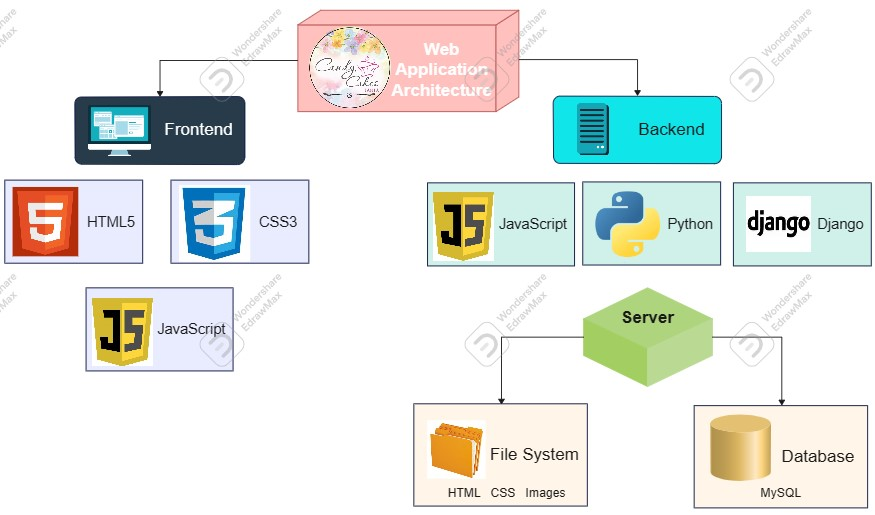
\includegraphics[width=0.8\linewidth]{./Arch.jpg}
\caption{"Candy Cakes" web application architecture}
\label{fig:overview}
\end{figure}




\subsection{Objectives}
Our website aims to make dealing with clients and owner easier by considering three questions:
\begin{itemize}
\item  What the client's needs when looking for products.
\item  what is the exact information we need to know about the client in order to complete the order faster and successfully.
\item  what is the best way to make an interesting website in order to attract the client's attention 
\end{itemize}
\subsection{Stakeholder}
\subsubsection{Internal}
Our team leader is Malak Mohammed Salem (21P0277), and the 
Team members are 
Hager Hesham (21P0297) ,
Malak mahmoud (21P0278) ,
Maryam Mahmoud (21P0214) ,and
Tsneam Ahmed Eliwa (21P0284).

\subsubsection{External}
The user of our website is Candy cake's owner and clients .

\section{Similar System}
\subsection{Academic}

List down at least 1 paper from ACM or IEEE for similar work experience in the domain of your problem. Be sure that each paper you list include the following points

\begin{enumerate}
\item The main problem statement of the work.
\item How the researchers contributed to solve the problem
\item The dataset used by the researchers
\item What main results the researchers reach.
\item Criticize the paper
\item Figure/s of the work (if available)
\end{enumerate}

\subsection{Business Applications}
Describe available business applications in the market with figures.
\begin{Business Applications}
\centering
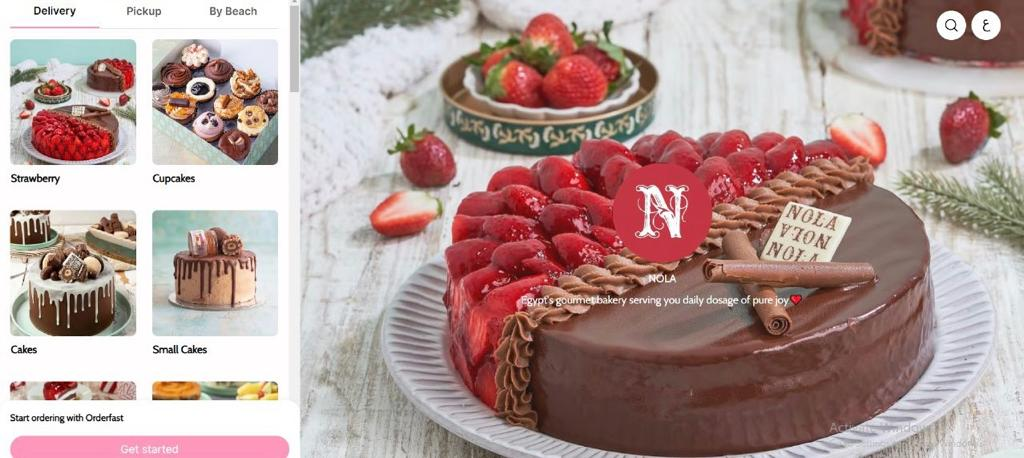
\includegraphics[width=0.6\linewidth]{Nola.jpg}


NOLA



\centering
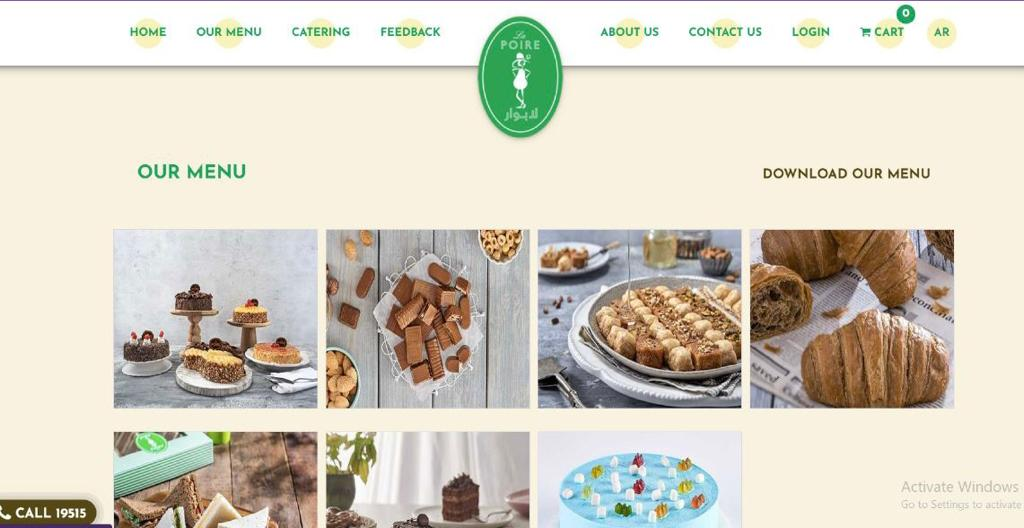
\includegraphics[width=0.6\linewidth]{LA poire.jpg}

La Poire

\end{Business Applications}




\section{Project Management and Deliverables}
\subsection{Deliverables}
\begin{itemize}
\item What will the project produce? (program, reports, etc.)
\item Describe in brief detail the features of each deliverable.
\end{itemize}
\subsection{Tasks and Time Plan}
Use \textcolor{blue}{\href{https://trello.com/power-ups/58bd1f9aca72f48c8900574f}{Trello}} to create a time plan showing tasks and which team member is assigned to it of your project.\\ 

\begin{figure}[h]
\centering
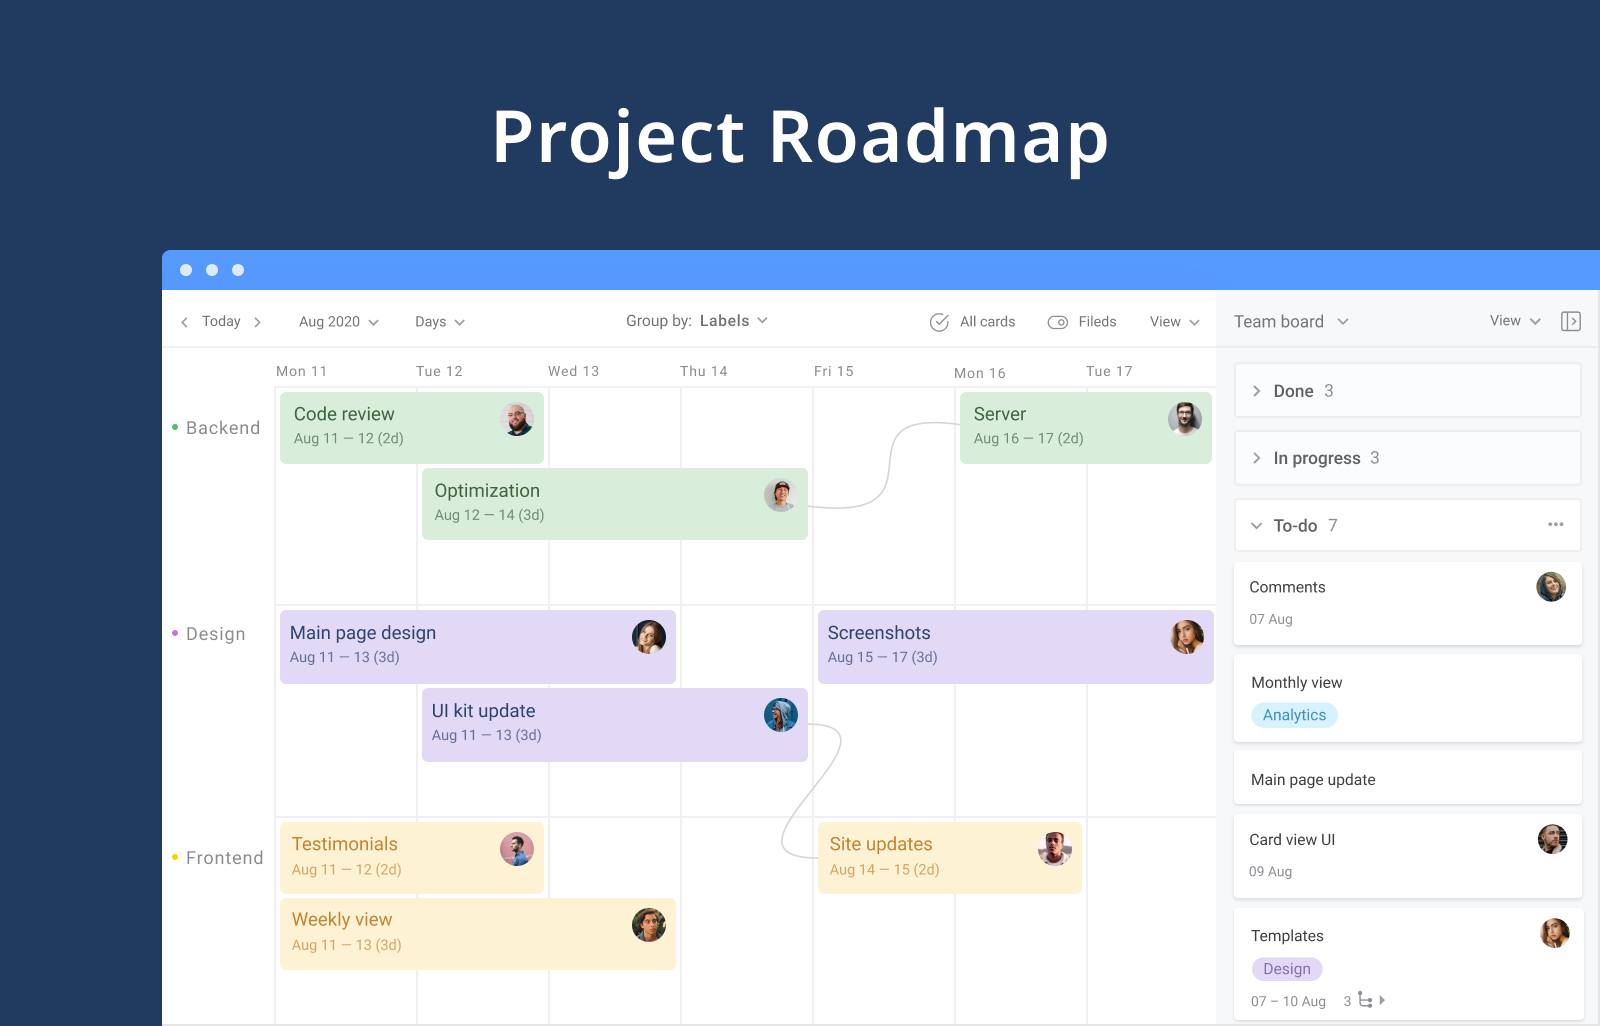
\includegraphics[width=0.8\linewidth]{images/trello_time_plan.png}
\caption{Project time plan}
\label{fig:timeplan}
\end{figure}
\newpage

\printbibliography
\end{document}
